\documentclass[a4paper, 12pt, titlepage]{report}

%Taal: Nederlands ("Inhoudsopgave", "Hoofdstuk",...)
\usepackage{graphicx}
\usepackage{subcaption}
\usepackage{algorithmic}
\usepackage{amsmath, amssymb, textcomp, mathtools}
\usepackage{mcode}

%Hyperlinks
\usepackage{hyperref}

%Opmaak hyperlinks
\hypersetup{colorlinks=false,	urlcolor=cyan,pdfborder=0 0 0}

%Geen nummering bij secties en hoofdstukkden
\setcounter{secnumdepth}{-1} 

%geen indents
\setlength\parindent{0pt}

\usepackage{listings}
\lstset{
language=Matlab, % choose the language of the code
%basicstyle=10pt, % the size of the fonts that are used for the code
numbers=left, % where to put the line-numbers
numberstyle=\footnotesize, % the size of the fonts that are used for the line-numbers
stepnumber=1, % the step between two line-numbers. If it's 1 each line will be numbered
numbersep=5pt, % how far the line-numbers are from the code
%backgroundcolor=\color{grey}, % choose the background color. You must add \usepackage{color}
showspaces=false, % show spaces adding particular underscores
showstringspaces=false, % underline spaces within strings
showtabs=false, % show tabs within strings adding particular underscores
frame=single, % adds a frame around the code
%tabsize=2, % sets default tabsize to 2 spaces
%captionpos=b, % sets the caption-position to bottom
breaklines=true, % sets automatic line breaking
breakatwhitespace=false, % sets if automatic breaks should only happen at whitespace
escapeinside={\%*}{*)} % if you want to add a comment within your code
}


%"Figuur" in vet
\makeatletter
\renewcommand{\fnum@figure}{\small\textbf{\figurename~\thefigure}}
\makeatother

\usepackage[dutch]{babel}
\begin{document}

\title{\textbf{Numerieke Modellering en Benadering}}
\author{De Wolf Peter\\ Vekemans Wout}

\date{\today}
\begin{titlepage}
	\maketitle
	\thispagestyle{empty}
\end{titlepage}

\newpage
\tableofcontents

\listoffigures

\newpage
\section{Benaderen met veeltermen}
In dit practicum willen we eerst enkele functies benaderen met behulp van veeltermen door interpolatie. We gebruiken hierto nulpunten van orthogonale veeltermen als interpolatiepunten.
\subsection{Berekenen van nulpunten van orthogonale veeltermen}
\lstinputlisting{poly_zeros.m}
Deze functie berekent de nulpunten van de orthogonale veeltermen gebaseerd op de waarden $\alpha_k, \beta_k$, en $\lambda_k$ uit de recursiebetrekking voor orthogonale veeltermen \eqref{recursion}. Het doet dit door een tridiagonale matrix op te stellen met elementen afgeleid van de co\"efficienten uit die recursiebetrekking. De nulpunten van de veelterm zijn dan gelijk aan de eigenwaarden van die matrix.\\
\begin{subequations} \label{recursion}
\begin{align}
\phi_0(x) = \lambda_0\; ;\; \phi_1(x) = \lambda_1(x-\alpha_1)\phi_0(x))\\
\phi_k(x) = \lambda_k(x-\alpha_k)\phi_{k-1}(x))-\beta_k\phi_{k-2}(x)
\end{align}
\end{subequations}

\subsection{Evauleren van drietermsrecursiebetrekking}
\lstinputlisting{eval_recursion.m}
Deze functie evalueert de drietermsrecursiebetrekking in de punten gegeven in de vector $x$. Als we deze methode toepassen op de 10 eerste Chebychev veeltermen krijgen we figuur \ref{chebychev}. Deze functie is eenvoudig toe te passen omdat Chebychev veeltermen duidelijk voldoen aan vergelijking \eqref{recursion}. Dit is makkelijk in te zien als men in de recursiebetrekking volgende waarden invult: $\lambda_0=1, \lambda_1=1$ en alle andere $\lambda_k$ gelijk aan 2. $\alpha_k$ is gelijk aan 0, en $\beta_k$ is 1. \\

\begin{figure}[htb]
	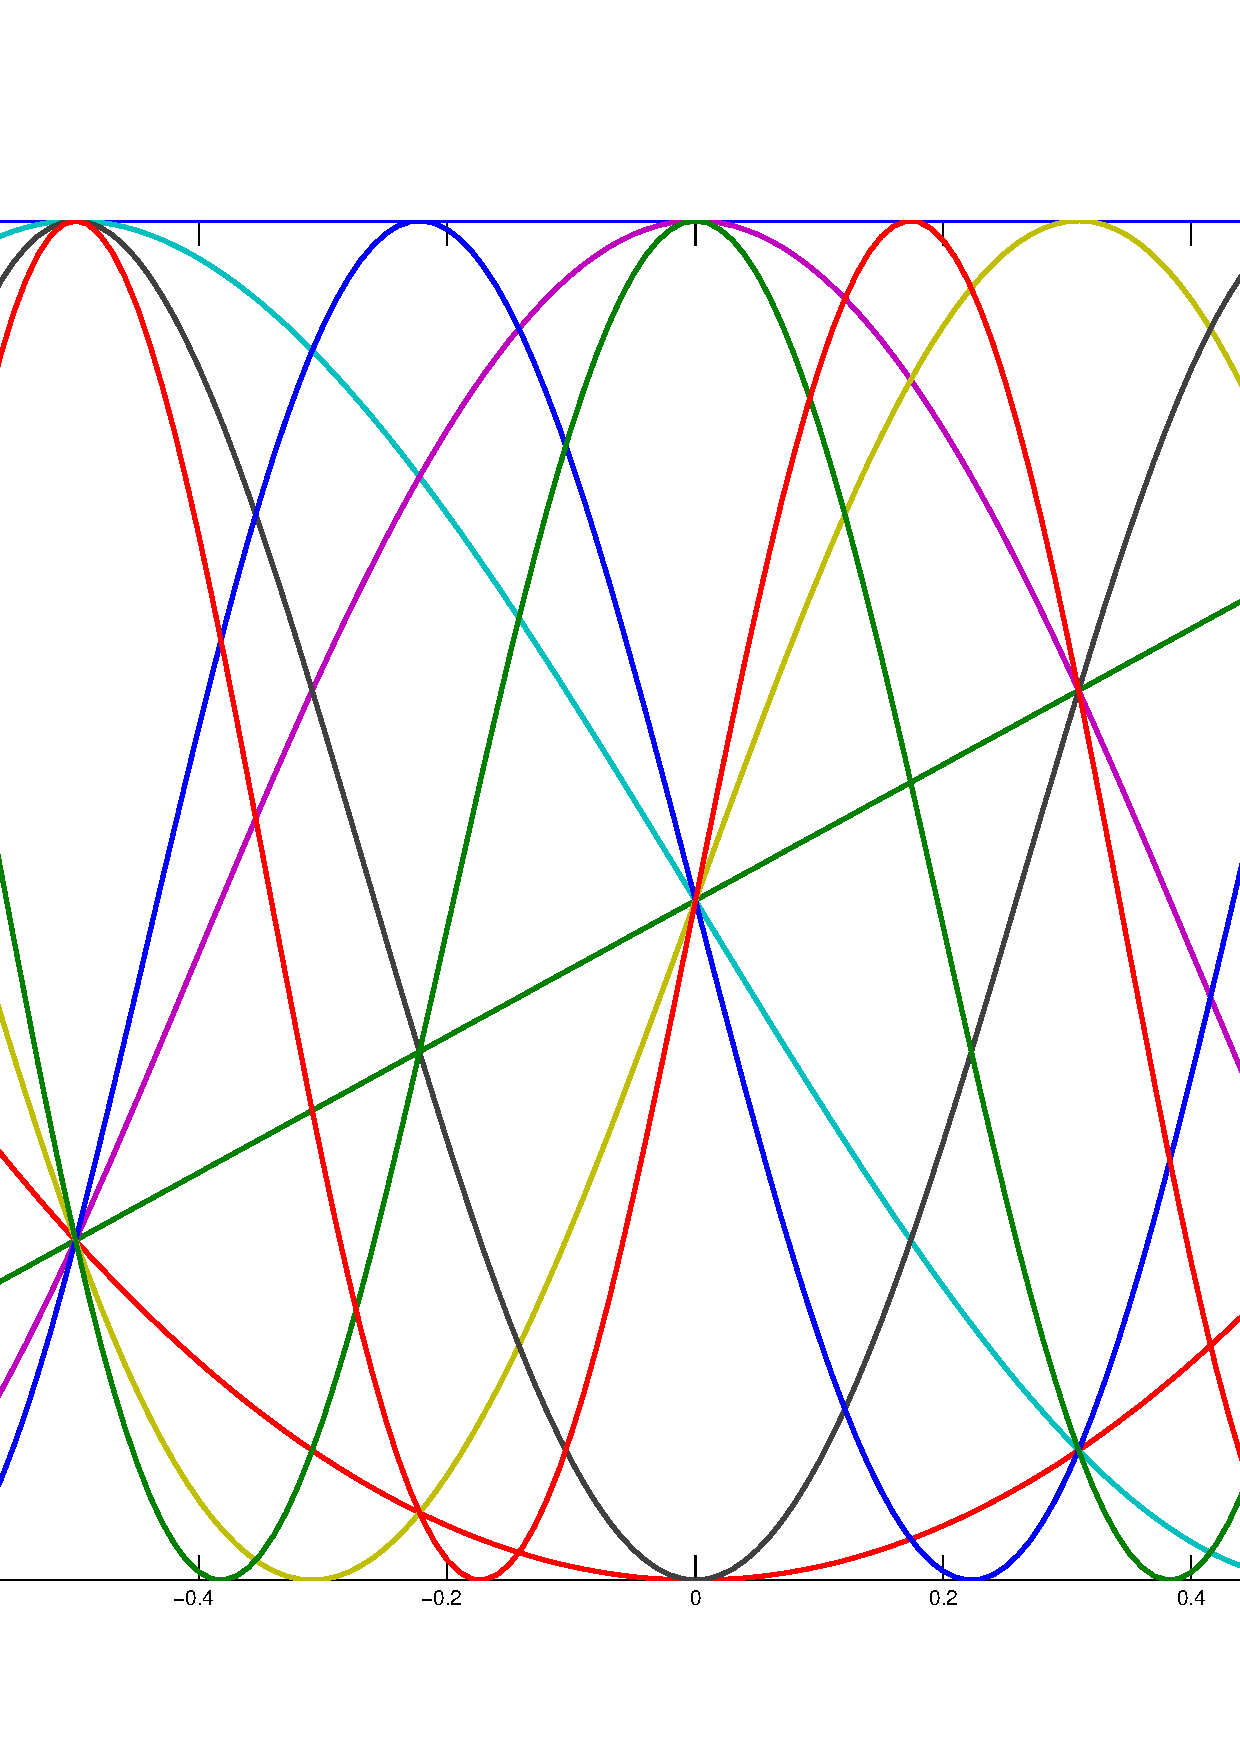
\includegraphics[width=\textwidth]{chebychev.png}
	\caption{Evaluatie van eerste tien Cheybchev veeltermen op 200 punten in [-1,1]}
	\label{chebychev}
\end{figure}
\section{Berekenen van interpolerende veelterm}
\begin{lstlisting}
function y = interpolate(x, f, alpha, beta, lambda, t)

%maak M matrix
M=eval_recursion(x,length(alpha),alpha,beta,lambda);

%bereken de coefficienten van de interpolerende veelterm
c=M\f;

%bereken de waarden van de interpolerende veelterm in t
values=eval_recursion(t,length(alpha),alpha,beta,lambda);
res=values*c;
\end{lstlisting}

Dit algoritme berekent een interpolerende veelterm door de waarden $f(x)$ en evalueert die veelterm in de punten gegeven in $t$. Als we dit toepassen op respectievelijk $\cos(x)$ en $\frac{1}{1+6x^2}$ krijgen we grafiek \ref{interpolcos} en \ref{interpolexp}. We zien op het eerste zicht niet duidelijk verschil tussen het gebruik van equidistante interpolatiepunten en de nulpunten van de Chebychev-veelterm $T_n$. Bij een verdere analyse van de interpolatiefout blijkt echter dat de nulpunten van de Chebychev veeltermen een veel beter gespreide fout geven. Voor illustratie, zie figuur \ref{errpolcos}. Bij de equidistante punten is er aan de rand van het interval een veel grotere fout aanwezig. Bij benaderingen van lagere graad is de absolute fout wel kleiner bij de equidistante punten.\\
 Als we de maximale fout in functie van de graad van de benadering uitzetten zien we ook dat bij hogere graad de equidistante punten weer onderdoen. We merken zelfs een stijging in de maximale fout vanaf een bepaald punt. De Chebychev interpolatie daarentegen daalt in het begin ongeveer even snel, maar blijft bij hogere graad constant rond $\epsilon_{mach}$. Dit wordt duidelijk op figuur \ref{maxerrcos}.\\

\begin{figure}[!h]
\begin{subfigure}{0.5\textwidth}
\centering
\includegraphics[width=\textwidth]{cosEqui.png}
\subcaption{Equidistant}
\end{subfigure}
\begin{subfigure}{0.5\textwidth}
\centering
\includegraphics[width=\textwidth]{cosCheb.png}
\subcaption{Nulpunten van $T_n$}
\end{subfigure}

\caption{Enkele interpolerende veeltermen van $\cos(x)$}
\label{interpolcos}
\end{figure}

\begin{figure}[!h]
\begin{subfigure}{\textwidth}
\centering
\includegraphics[width=\textwidth]{errorCos1.png}
\subcaption{Equidistant}
\end{subfigure}
\begin{subfigure}{\textwidth}
\centering
\includegraphics[width=\textwidth]{errorCos2.png}
\subcaption{Nulpunten van $T_n$}
\end{subfigure}

\caption{Absolute fout bij het interpoleren van $\cos(x)$}
\label{errpolcos}
\end{figure}

\begin{figure}[htb]
	\centering
	\includegraphics[width=\textwidth]{maxCos.png}
	\caption{Maximale interpolatiefout voor beide methoden}
	\label{maxerrcos}
\end{figure}
\end{document}